\chapter{The Qubit: Beyond the Bit}\label{ch:qubit}
\begin{center}\small\textit{From 0-or-1 to $\alpha\lvert0\rangle+\beta\lvert1\rangle$ --- why nature's bit is a sphere, not a switch.}\end{center}

\section{Intuition: Why a Bit Is Not Enough}
A classical bit is a switch: OFF is 0, ON is 1. Every computer you have used stores essays, photos and videos as strings of such switches. This picture is powerful but incomplete --- it describes what we \emph{engineered}, not what nature \emph{allows}.

Quantum mechanics says a particle (an electron spin, a photon polarization, a superconducting loop) can be in a \emph{superposition}: partly 0 and partly 1 at once, with weights that are complex numbers. Until you look, the system \emph{is} both. When you do look, nature rolls dice: you see 0 with some probability, 1 otherwise, and the superposition is gone. This randomness is not ignorance --- it is how the world works at small scales.

The qubit is the mathematical model of this idea. It keeps the case ``0 or 1'' but upgrades the state space from two points to a whole continuum.

\section{Formalism: The Qubit}
We work in $\mathbb{C}^2$ with computational basis
\begin{equation}
\lvert0\rangle=\begin{pmatrix}1\\0\end{pmatrix},\qquad
\lvert1\rangle=\begin{pmatrix}0\\1\end{pmatrix}.
\end{equation}

\begin{definition}[Qubit]
A (pure) qubit state is a unit vector
\begin{equation}
\lvert\psi\rangle = \alpha\lvert0\rangle+\beta\lvert1\rangle,\qquad
\alpha,\beta\in\mathbb{C},\quad |\alpha|^2+|\beta|^2=1 .
\end{equation}
$|\alpha|^2$ is the probability of measuring $0$, $|\beta|^2$ of measuring $1$. Global phase is unphysical: $e^{i\gamma}\lvert\psi\rangle\equiv\lvert\psi\rangle$.
\end{definition}

Writing $\alpha=\cos\frac{\theta}{2}$ and $\beta=e^{i\varphi}\sin\frac{\theta}{2}$ with $\theta\in[0,\pi]$, $\varphi\in[0,2\pi)$ gives the Bloch representation. Every pure state is a point on the unit sphere.

\begin{definition}[Bloch sphere]
The map $\lvert\psi\rangle\mapsto \mathbf{r}=(\sin\theta\cos\varphi,\sin\theta\sin\varphi,\cos\theta)\in S^2$ is a bijection between pure qubit states modulo phase and points on the Bloch sphere. North pole $=\lvert0\rangle$, south pole $=\lvert1\rangle$, equator $=$ equal superposition.
\end{definition}

\begin{center}
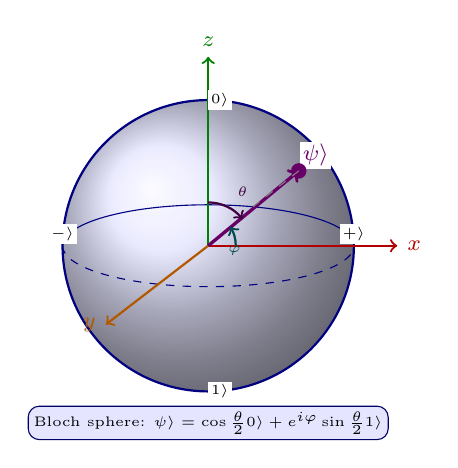
\begin{tikzpicture}[scale=1.0,font=\footnotesize]
  % Sphere shading
  \shade[ball color=blue!12, opacity=0.9] (0,0) circle (1.85cm);
  \draw[thick, blue!50!black] (0,0) circle (1.85cm);
  \draw[blue!50!black, dashed] (-1.85,0) arc (180:360:1.85 and 0.52);
  \draw[blue!50!black] (-1.85,0) arc (180:0:1.85 and 0.52);
  % Axes
  \draw[->, thick, red!70!black] (0,0)--(2.4,0) node[right] {$x$};
  \draw[->, thick, green!50!black] (0,0)--(0,2.4) node[above] {$z$};
  \draw[->, thick, orange!70!black] (0,0)--(-1.3,-1.0) node[left] {$y$};
  % State vector
  \coordinate (psi) at (1.15,0.95);
  \draw[->, very thick, violet!80!black] (0,0)--(psi) node[above right, fill=white, inner sep=1pt] {$\lvert\psi\rangle$};
  \fill[violet!80!black] (psi) circle (2.8pt);
  % Angles
  \draw[->, thick, violet!50!black] (0,0.55) arc (90:38:0.55) node[midway, above right, font=\tiny] {$\theta$};
  \draw[->, thick, teal!60!black] (0.35,0) arc (0:32:0.45) node[midway, below, font=\tiny] {$\varphi$};
  \draw[dashed, gray] (psi)--(0.55,0.48);
  \node[fill=blue!10,draw=blue!40!black,rounded corners,inner sep=2pt, font=\tiny] at (0,-2.25) {Bloch sphere: $\lvert\psi\rangle=\cos\frac{\theta}{2}\lvert0\rangle+e^{i\varphi}\sin\frac{\theta}{2}\lvert1\rangle$};
  \node[font=\tiny, fill=white, inner sep=1pt] at (0.15,1.85) {$\lvert0\rangle$};
  \node[font=\tiny, fill=white, inner sep=1pt] at (0.15,-1.85) {$\lvert1\rangle$};
  \node[font=\tiny, fill=white, inner sep=1pt] at (1.85,0.15) {$\lvert+\rangle$};
  \node[font=\tiny, fill=white, inner sep=1pt] at (-1.85,0.15) {$\lvert-\rangle$};
\end{tikzpicture}
\end{center}

Measurement in the computational basis projects onto $\lvert0\rangle$ or $\lvert1\rangle$ (Born rule). Measuring a different basis corresponds to rotating the sphere first. Concretely, measuring
$\lvert+\rangle=\tfrac{\lvert0\rangle+\lvert1\rangle}{\sqrt2}$ vs.\ $\lvert-\rangle=\tfrac{\lvert0\rangle-\lvert1\rangle}{\sqrt2}$
is an $X$-basis measurement.

\begin{center}
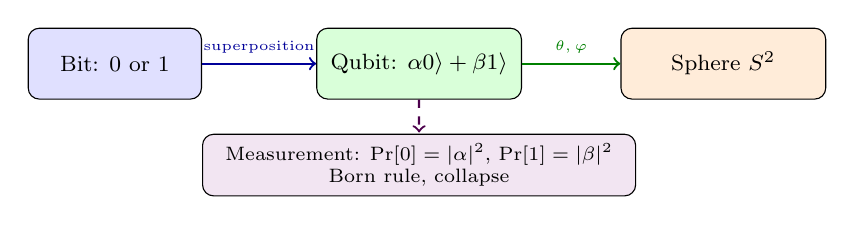
\begin{tikzpicture}[scale=0.92,font=\footnotesize]
  \node[draw, fill=blue!12, rounded corners, minimum width=2.2cm, minimum height=0.9cm] (b) at (0,0) {Bit: $0$ or $1$};
  \node[draw, fill=green!15, rounded corners, minimum width=2.6cm, minimum height=0.9cm] (q) at (4.2,0) {Qubit: $\alpha\lvert0\rangle+\beta\lvert1\rangle$};
  \node[draw, fill=orange!15, rounded corners, minimum width=2.6cm, minimum height=0.9cm] (s) at (8.4,0) {Sphere $S^2$};
  \draw[->, thick, blue!60!black] (b)--(q) node[midway, above, font=\tiny] {superposition};
  \draw[->, thick, green!50!black] (q)--(s) node[midway, above, font=\tiny] {$\theta,\varphi$};
  % probabilities
  \node[draw, fill=violet!10, rounded corners, minimum width=5.5cm, align=center, font=\scriptsize] at (4.2,-1.4) {Measurement: $\Pr[0]=|\alpha|^2$, $\Pr[1]=|\beta|^2$\\Born rule, collapse};
  \draw[->, thick, violet!60!black, dashed] (q)--(4.2,-0.95);
\end{tikzpicture}
\end{center}

\section{Measurement and Collapse}
\begin{theorem}[Born rule + collapse]
Measuring $\lvert\psi\rangle=\alpha\lvert0\rangle+\beta\lvert1\rangle$ in basis $\{\lvert0\rangle,\lvert1\rangle\}$ yields outcome $0$ with probability $|\alpha|^2$ leaving state $\lvert0\rangle$, and outcome $1$ with probability $|\beta|^2$ leaving $\lvert1\rangle$.
\end{theorem}

Repeated preparation and measurement estimates $|\alpha|,|\beta|$ but single-shot measurement cannot learn both amplitudes --- a \emph{no-cloning} hint. Relative phase $\varphi$ is invisible in $Z$-basis statistics but appears in $X$-basis:
\begin{equation}
\Pr[+]=|\langle+\vert\psi\rangle|^2=\tfrac12+\mathrm{Re}(\alpha^*\beta),\;
\Pr[-]=\tfrac12-\mathrm{Re}(\alpha^*\beta).
\end{equation}

\begin{example}[Interference]
$\lvert\psi_1\rangle=\tfrac{\lvert0\rangle+\lvert1\rangle}{\sqrt2}$ and $\lvert\psi_2\rangle=\tfrac{\lvert0\rangle-\lvert1\rangle}{\sqrt2}$ give identical $Z$ statistics (50/50) but opposite $X$ statistics. Phase matters --- it is how quantum algorithms create constructive and destructive interference.
\end{example}

\section{Multi-Qubit Preview}
Two qubits live in $\mathbb{C}^4$ with basis $\lvert00\rangle,\lvert01\rangle,\lvert10\rangle,\lvert11\rangle$. A general state $\sum_{x\in\{0,1\}^2}c_x\lvert x\rangle$ has $4$ amplitudes; $n$ qubits have $2^n$. This exponential Hilbert space is the source of quantum power --- and of simulation hardness.

\begin{center}
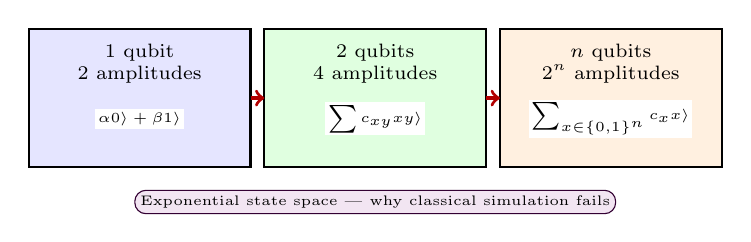
\begin{tikzpicture}[scale=0.88,font=\footnotesize]
  \fill[blue!10] (0,0) rectangle (3.2,2.0);
  \fill[green!12] (3.4,0) rectangle (6.6,2.0);
  \fill[orange!12] (6.8,0) rectangle (10.0,2.0);
  \draw[thick] (0,0) rectangle (3.2,2.0);
  \draw[thick] (3.4,0) rectangle (6.6,2.0);
  \draw[thick] (6.8,0) rectangle (10.0,2.0);
  \node[align=center, font=\scriptsize] at (1.6,1.5) {1 qubit\\2 amplitudes};
  \node[align=center, font=\scriptsize] at (5.0,1.5) {2 qubits\\4 amplitudes};
  \node[align=center, font=\scriptsize] at (8.4,1.5) {$n$ qubits\\$2^n$ amplitudes};
  \node[font=\tiny, fill=white, inner sep=1pt] at (1.6,0.7) {$\alpha\lvert0\rangle+\beta\lvert1\rangle$};
  \node[font=\tiny, fill=white, inner sep=1pt] at (5.0,0.7) {$\sum c_{xy}\lvert xy\rangle$};
  \node[font=\tiny, fill=white, inner sep=1pt] at (8.4,0.7) {$\sum_{x\in\{0,1\}^n}c_x\lvert x\rangle$};
  \draw[->, very thick, red!70!black] (3.2,1.0)--(3.4,1.0);
  \draw[->, very thick, red!70!black] (6.6,1.0)--(6.8,1.0);
  \node[fill=violet!10, draw=violet!40!black, rounded corners, inner sep=2pt, font=\tiny] at (5.0,-0.5) {Exponential state space --- why classical simulation fails};
\end{tikzpicture}
\end{center}

\section{Python: Qubits with NumPy}

\begin{lstlisting}[language=Python]
import numpy as np

# |0>, |1>, |+>, |-> as vectors
ket0 = np.array([1,0], dtype=complex)
ket1 = np.array([0,1], dtype=complex)
ket_plus = (ket0 + ket1)/np.sqrt(2)
ket_minus = (ket0 - ket1)/np.sqrt(2)

def qubit(alpha, beta):
    """Create normalized qubit a|0>+b|1>."""
    v = np.array([alpha, beta], dtype=complex)
    return v / np.linalg.norm(v)

def bloch_coords(state):
    """Return (x,y,z) Bloch vector for pure state."""
    a, b = state
    x = 2*np.real(np.conj(a)*b)
    y = 2*np.imag(np.conj(a)*b)
    z = np.abs(a)**2 - np.abs(b)**2
    return (x, y, z)

def measure_probs(state):
    """Born rule probabilities in Z basis."""
    return np.abs(state)**2  # [P0, P1]

# Example: Hadamard state and measurement
psi = qubit(1, 1)  # |+>
print("psi =", psi)
print("Bloch:", bloch_coords(psi))     # ~(1,0,0)
print("P0,P1 :", measure_probs(psi))   # [0.5, 0.5]
# X-basis probability: |<+|psi>|^2
p_plus = abs(np.vdot(ket_plus, psi))**2
print("P(+) in X-basis:", p_plus)
\end{lstlisting}

\begin{lstlisting}[language=Python]
# Simulate measurement collapse (Monte Carlo)
import random

def measure(state, shots=1000):
    p0 = abs(state[0])**2
    counts = {"0": 0, "1": 0}
    for _ in range(shots):
        counts["0" if random.random() < p0 else "1"] += 1
    return counts

psi = qubit(np.cos(0.6), np.exp(1j*0.7)*np.sin(0.6))
print("psi Bloch:", bloch_coords(psi))
print(measure(psi, 2000))

# Verify normalization and global phase invariance
phase = np.exp(1j*1.23)
psi2 = phase * psi
print("Same Bloch after phase?",
      np.allclose(bloch_coords(psi), bloch_coords(psi2)))
\end{lstlisting}


\section{Density Matrices and Global Phase}
For completeness, a mixed state $\rho=\sum_i p_i\lvert\psi_i\rangle\langle\psi_i\rvert$ has $\mathrm{Tr}\,\rho=1$, $\rho\succeq0$, $\mathrm{Tr}\,\rho^2\le1$ with equality iff pure. Bloch form for any single-qubit state is
\begin{equation}
\rho=\tfrac12\bigl(I+xX+yY+zZ\bigr),\quad x^2+y^2+z^2\le1,
\end{equation}
so interior of sphere $=$ mixed states. Pure states are surface points. Global phase $e^{i\gamma}$ cancels in $\rho=\lvert\psi\rangle\langle\psi\rvert$, explaining its unphysical nature. The fidelity between $\rho$ and $\sigma$ is $F=\bigl(\mathrm{Tr}\sqrt{\sqrt\rho\,\sigma\sqrt\rho}\bigr)^2$, reducing to $|\langle\psi|\phi\rangle|^2$ for pure states.
\begin{remark}
Relative phase is physical because it changes $\rho$. Example: $\lvert+\rangle\langle+\rvert\neq\lvert-\rangle\langle-\rvert$ though both are $50/50$ in $Z$ basis. This is why interferometers sense phase.
\end{remark}

\section{Exercises}
\begin{exercise}
Normalize $\lvert\phi\rangle= (1+i)\lvert0\rangle + (2-i)\lvert1\rangle$ and find $\Pr[0]$, $\Pr[1]$ and its Bloch coordinates $(\theta,\varphi)$.
\end{exercise}
\begin{exercise}
Show that $\lvert+\rangle$ and $\lvert-\rangle$ are orthogonal and each lies on the Bloch equator. Which $(\theta,\varphi)$ correspond to $\lvert+i\rangle=\tfrac{\lvert0\rangle+i\lvert1\rangle}{\sqrt2}$?
\end{exercise}
\begin{exercise}
Prove global phase is unphysical: for any measurement basis $\{\lvert m\rangle\}$, $|\langle m\vert\psi\rangle|^2=|\langle m|e^{i\gamma}\psi\rangle|^2$. Find a relative phase that \emph{does} change $X$-basis statistics.
\end{exercise}
\begin{exercise}
A qubit is measured in $Z$ basis with outcome $0$ with probability $3/4$. Give all possible states (up to global phase) and their Bloch $z$-coordinates.
\end{exercise}
\begin{exercise}
Write a Python function that, given $n$, builds the $2^n$-dimensional state vector for $\lvert+\rangle^{\otimes n}$ and verifies that every amplitude equals $2^{-n/2}$. Test for $n=3$.
\end{exercise}
